\documentclass[12pt]{article}

\title{Activity 1: Introduction}
\author{Chris Mayfield and Helen Hu}
\date{July 2017}

%\ProvidesPackage{cspogil}

% fonts
\usepackage[utf8]{inputenc}
\usepackage[T1]{fontenc}
\usepackage{mathpazo}

% spacing
\usepackage[margin=2cm]{geometry}
\renewcommand{\arraystretch}{1.4}
\setlength{\parindent}{0pt}

% orphans and widows
\clubpenalty=10000
\widowpenalty=10000
\pagestyle{empty}

% figures and tables
\usepackage{graphicx}
\usepackage{multicol}
\usepackage{tabularx}
\usepackage{wrapfig}

% fixed-width columns
\usepackage{array}
\newcolumntype{L}[1]{>{\raggedright\let\newline\\\arraybackslash\hspace{0pt}}m{#1}}
\newcolumntype{C}[1]{>{\centering\let\newline\\\arraybackslash\hspace{0pt}}m{#1}}
\newcolumntype{R}[1]{>{\raggedleft\let\newline\\\arraybackslash\hspace{0pt}}m{#1}}

% include paths
\makeatletter
\def\input@path{{Models/}{../../Models/}}
\graphicspath{{Models/}{../../Models/}}
\makeatother

% colors
\usepackage[svgnames,table]{xcolor}
\definecolor{bgcolor}{HTML}{FAFAFA}
\definecolor{comment}{HTML}{007C00}
\definecolor{keyword}{HTML}{0000FF}
\definecolor{strings}{HTML}{B20000}

% table headers
\newcommand{\tr}{\bf\cellcolor{Yellow!10}}

% syntax highlighting
\usepackage{textcomp}
\usepackage{listings}
\lstset{
    basicstyle=\ttfamily\color{black},
    backgroundcolor=\color{bgcolor},
    numberstyle=\scriptsize\color{comment},
    commentstyle=\color{comment},
    keywordstyle=\color{keyword},
    stringstyle=\color{strings},
    columns=fullflexible,
    keepspaces=true,
    showlines=true,
    showstringspaces=false,
    upquote=true
}

% code environments
\newcommand{\java}[1]{\lstinline[language=java]{#1}}%[
\lstnewenvironment{javalst}{\lstset{language=java,backgroundcolor=}}{}
\lstnewenvironment{javabox}{\lstset{language=java,frame=single,numbers=left}\quote}{\endquote}

% PDF properties
\usepackage[pdftex]{hyperref}
\urlstyle{same}
\makeatletter
\hypersetup{
  pdftitle={\@title},
  pdfauthor={\@author},
  pdfsubject={\@date},
  pdfkeywords={},
  bookmarksopen=false,
  colorlinks=true,
  citecolor=black,
  filecolor=black,
  linkcolor=black,
  urlcolor=blue
}
\makeatother

% titles
\makeatletter
\renewcommand{\maketitle}{\begin{center}\LARGE\@title\end{center}}
\makeatother

% boxes [optional height]
\newcommand{\emptybox}[1][10em]{
\vspace{1em}
\begin{tabularx}{\linewidth}{|X|}
\hline\\[#1]\hline
\end{tabularx}}

% models
\newcommand{\model}[1]{\section{#1}\nopagebreak}
\renewcommand{\thesection}{Model~\arabic{section}}

% questions
\newcommand{\quest}[1]{\subsection*{Questions~ (#1)}}
\newcounter{question}
\newcommand{\Q}{\vspace{1em}\refstepcounter{question}\arabic{question}.~ }
\renewcommand{\thequestion}{\#\arabic{question}}

% sub-question lists
\usepackage{enumitem}
\setenumerate[1]{label=\alph*)}
\setlist{itemsep=1em,after=\vspace{1ex}}

% inline answers
\definecolor{answers}{HTML}{C0C0C0}
\newcommand{\ans}[1]{%
\ifdefined\Student
    \leavevmode\phantom{~~\textcolor{answers}{#1}}
\else
    ~~\textcolor{answers}{#1}
\fi}

% longer answers [optional height]
\newsavebox{\ansbox}
\newenvironment{answer}[1][4em]{
\nopagebreak
\begin{lrbox}{\ansbox}
\begin{minipage}[t][#1]{\linewidth}
\color{answers}
}{
\end{minipage}
\end{lrbox}
\ifdefined\Student
    \phantom{\usebox{\ansbox}}%
\else
    \usebox{\ansbox}%
\fi}


\begin{document}

\maketitle

In this course, you will work in teams of 3--4 students to learn new concepts.
This activity will introduce you to the process.
We'll also take a first look at how to store data in Java programs.

\guide{
  \item Describe the responsibility of each POGIL role.
  \item Identify components of the "hello world" program.
  \item Write Java code to declare int and double variables.
  \item Explain what it means to assign a value to a variable.
}{
  \item Leveraging prior knowledge and experience of other students. (Teamwork)
}{
This activity is designed for the first day or week of CS1. There are no prerequisites. As the first activity, it's important to explain/model the instructor's role in a POGIL classroom. For large classes, it may take a bit longer than expected to organize teams.

\ref{team-roles.tex} refers to \github{Handouts/role-cards-mayfield.pdf}{Role Cards}, which ideally should be printed out on a different color of card stock (one set per team). You may also want to have each team complete a \github{Handouts/reflectors-report.pdf}{Reflector's Report} for this activity.

One strategy for reporting out \ref{hello-world.tex} is to have presenters of nearby teams swap answers and discuss any differences. Introduce the terms \emph{documentation} (see \ref{javadoc}) and \emph{newline} (see \ref{println}).

\ref{vardecl} and \ref{xgets} are good for reporting out. It's important that teams hear multiple perspectives on these concepts. Introduce the terms \emph{data type} and \emph{operator}, and point out that \emph{assignment} is not the same as \emph{equality}.

On \ref{assignment.tex}, it may be necessary to explain that there are only two variables. The boxes show the state of memory over time, as the corresponding statements are executed.
}

\section*{Meta Activity: Team Roles}

Decide who will be what role for today; we will rotate the roles each week.
If you have only three people, one should have two roles.
If you have five people, two may share the same role.

\begin{table}[h!]
\renewcommand{\arraystretch}{1.6}
\begin{tabular}{|p{0.45\linewidth}|p{0.50\linewidth}}
\cline{1-1}

Manager:
\hfill \ans[13em]{Helen Hu}       & ~~ \ans[19em]{keeps track of time, all voices are heard}
\\ \cline{1-1}

Presenter:
\hfill \ans[13em]{Clif Kussmaul}  & ~~ \ans[19em]{asks questions, gives the team's answers}
\\ \cline{1-1}

Recorder:
\hfill \ans[13em]{Chris Mayfield} & ~~ \ans[19em]{quality control and consensus building}
\\ \cline{1-1}

Reflector:
\hfill \ans[13em]{Aman Yadav}     & ~~ \ans[19em]{team dynamics, suggest improvements}
\\ \cline{1-1}

\end{tabular}
\end{table}


\quest{15 min}


\Q What is the difference between \textbf{bold} and \textit{italics} on the role cards?

\begin{answer}
The bold points describe what the responsibilities are.
Examples of what that person would say are in italics.
\end{answer}


\Q Manager: invite each person to explain their role to the team.
Recorder: take notes of the discussion by writing down key phrases next to the table above.

\vspace{1ex}


\Q What responsibilities do two or more roles have in common?

\begin{answer}
Both the presenter and the recorder help the team reach consensus.
The manager and reflector both monitor how the team is working.
\end{answer}


\Q For each role, give an example of how someone observing your team would know that a person is \underline{not} doing their job well.

\begin{itemize}

\item Manager:
\hfill \ans[33em]{The team is constantly getting behind.}

\item Presenter:
\hfill \ans[33em]{The student doesn't know what to say.}

\item Recorder:
\hfill \ans[33em]{Some team members aren't taking good notes.}

\item Reflector:
\hfill \ans[33em]{The student never comments on team dynamics.}

\end{itemize}

\model{Hello, World!}

\begin{center}
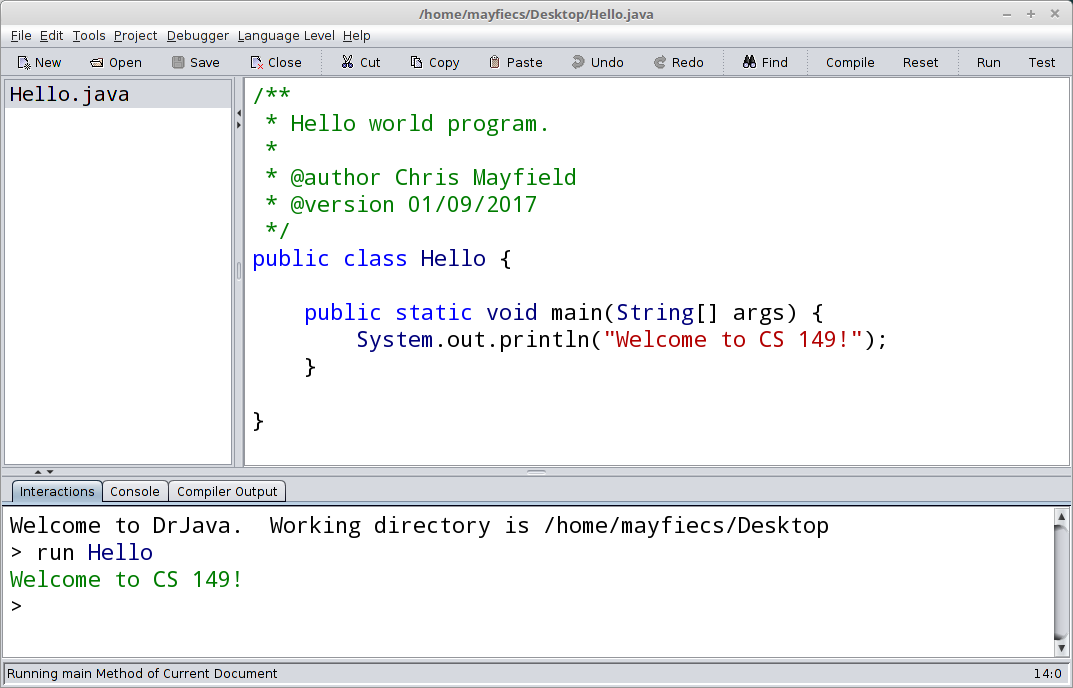
\includegraphics[height=3.65in]{drjava.png}
\end{center}


\quest{8 min}


\Q What is the name of the class?
What is the name of the file?
What directory is it in?

\begin{answer}
Class name: \texttt{Hello} ~~~
File name: \texttt{Hello.java} ~~~
Directory: \texttt{/home/mayfiecs/Desktop}
\end{answer}


\Q How many lines of code is the above program?
How many statements does it have?

\begin{answer}
The source file has 13 lines.
There is only one statement (the \java{System.out.println}).
\end{answer}


\Q What is the purpose of the first six lines?
What is the purpose of the two blank lines?

\begin{answer}
The first six lines describe what the program does and who wrote it.
The two blank lines make it easier to read the program (and are ignored).
\end{answer}


\Q Describe in your own words what \java{System.out.println} does.
Be very specific.

\begin{answer}
The \java{println} method displays a message on the screen, followed by a newline character.
When you run the \java{Hello} program, it prints a welcome message.
\end{answer}

\model{Variables}
% Based on Model 1 of "Activity 02 - Declaration and Assignments" by Helen Hu

Most programs store and manipulate data values, and we use \textit{variables} to give them meaningful names.
The following code \emph{declares} and \emph{assigns} three variables.
Each variable is stored in the computer's memory, represented by the boxes on the right.

\vspace{1em}
\hfill
\begin{minipage}[t]{0.5\textwidth}

\textbf{Java code}
\vspace{1ex}

\begin{javalst}
int dollars;
int cents;
double grams;

dollars = 1;
cents = 90;
grams = 3.5;
\end{javalst}

\end{minipage}
\hfill
\begin{minipage}[t]{0.4\textwidth}

\textbf{Computer memory}
\vspace{1em}

\var{dollars}{1}
\par\vspace{1em}
\var{cents}{90}
\par\vspace{1em}
\var{grams}{3.5}

\end{minipage}


\quest{10 min}


\Q Identify the Java \emph{keyword} used in a variable declaration to indicate

\begin{enumerate}
\item an integer: \ans{int}
\item a real number: \ans{double}
\end{enumerate}


\Q Consider numbers of dollar bills, cents, and grams.
Which of these units only makes sense as an integer, and why?

\begin{answer}
Cents makes sense (ha ha) only as an integer, because at the end of the day, you can't pay with a fractional amount. (It is possible to make a similar argument for dollars, but not for grams.)
\end{answer}


\Q What would you expect the following statements to print out?

\begin{enumerate}
\item \java{System.out.println(dollars);} \ans{1}
\item \java{System.out.println(cents);} \ans{90}
\item \java{System.out.println(grams);} \ans{3.5}
\end{enumerate}


\Q In the previous question, how does the third printed line (c) differ from the first two?

\begin{answer}
The third line prints a double, and the first two print an integer.
\end{answer}


\Q \label{vardecl}
What do you think is the purpose of a variable declaration?

\begin{answer}
It tells the computer how to interpret and display the value.
\end{answer}


\Q What is output by the following code, and why?

\begin{minipage}[t]{0.33\linewidth}

\vspace{-2ex}
\begin{javalst}
double one;
one = 1;
System.out.println(one);
\end{javalst}

\end{minipage}
\hfill
\begin{minipage}[t]{0.66\linewidth}

\begin{answer}
The output is 1.0, because {\tt one} is a {\tt double}.
The type of variable determines the output format.
\end{answer}

\end{minipage}

\smallskip
\model{Assignment}
% based on Model 2 of Activity 08 - Introduction to Loops by Helen Hu

Consider the following Java statements. What is the resulting value of each variable?

\begin{center}
\vspace{-6pt}
\begin{tabular}{cp{120pt}cp{120pt}cp{120pt}}

\textsf{A:}
&
\vspace{-1em}
\begin{javalst}
int x, y;
x = 1;
y = 2;
y = x;
x = y;

\end{javalst}

&
\textsf{B:}
&
\vspace{-1em}
\begin{javalst}
int x, y, z;
x = 1;
y = 2;
z = y;
y = x;
x = z;
\end{javalst}

&
\textsf{C:}
&
\vspace{-1em}
\begin{javalst}
int z, y;
z = 2;
z = z + 1;
z = z + 1;
y = y + 1;

\end{javalst}

\\[-1em]
&
Value of x: \ans[3em]{1}

\vspace{1em}
Value of y: \ans[3em]{1}

&
&
Value of x: \ans[3em]{2}

\vspace{1em}
Value of y: \ans[3em]{1}

\vspace{1em}
Value of z: \ans[3em]{2}

&
&
Value of z: \ans[3em]{4}

\vspace{1em}
Value of y: \ans[3em]{?}

\end{tabular}
\vspace{-14pt}
\end{center}


\quest{10 min}


\Q In program~\textsf{A}, why is the value of \java{x} not 2?

\begin{answer}[3em]
Each statement is executed one after the other, so the third assignment changes the value of \java{y} to 1.
The last assignment then assigns 1 to the value \java{x}.
\end{answer}


\Q In program~\textsf{B}, what happens to the values of \java{x} and \java{y}?

\begin{answer}[3em]
They get swapped; \java{x} was 1 and \java{y} was 2, but in the end \java{x} was 2 and \java{y} was 1.
\end{answer}


\Q In program~\textsf{B}, what is the purpose of the variable \java{z}?

\begin{answer}[3em]
It is a temporary variable that makes it possible to swap the values of \java{x} and \java{y}.
\end{answer}


\Q If program~\textsf{C} runs, what happens to the value of \java{z}?

\begin{answer}[3em]
It gets incremented twice; the value starts at 2, then it becomes 3, and then it becomes 4.
\end{answer}


\Q In program~\textsf{C}, why is it possible to increment \java{z} but not \java{y}?

\begin{answer}[3em]
The variable \java{z} was initialized, but \java{y} was not.
Java doesn't know what value to increment.
\end{answer}


\Q Because \emph{increment} and \emph{decrement} are so common in algorithms, Java provides the operators \java{++} and \java{--}.
For example, ~\java{x++} is the same as ~\java{x = x + 1}, and \java{y--} is the same as ~\java{y = y - 1}.
Write the value of \java{x} and \java{y} next to each statement below.

\vspace{-1ex}
\begin{center}
\begin{minipage}{90pt}
\begin{javalst}
int x = 5;
x--;
x--;
\end{javalst}
\end{minipage}
\begin{minipage}{100pt}
\begin{answer}[3.5em]
\begin{javaans}
x is 5
x is 4
x is 3
\end{javaans}
\end{answer}
\end{minipage}
\hspace{3em}
\begin{minipage}{90pt}
\begin{javalst}
int y = -10;
y++;
y++;
\end{javalst}
\end{minipage}
\begin{minipage}{100pt}
\begin{answer}[3.5em]
\begin{javaans}
y is -10
y is -9
y is -8
\end{javaans}
\end{answer}
\end{minipage}
\end{center}
\vspace{-1em}


\Q \label{compound}
Like the assignment operator, the \java{++} and \java{--} operators replace the value of a variable.
Java also has \emph{compound assignment} operators for convenience.
For example, the statement ~\java{x = x + 2} can be rewritten as ~\java{x += 2}.
Simplify the following assignment statements.

\vspace{-1ex}
\begin{center}
\begin{minipage}{150pt}
\begin{javalst}
step = step + 5;
size = size - 3;
total = total * 2;
change = change / 10;
hours = hours % 24;
\end{javalst}
\end{minipage}
\begin{minipage}{150pt}
\begin{answer}[6em]
\begin{javaans}
step += 5;
size -= 3;
total *= 2;
change /= 10;
hours %= 24;
\end{javaans}
\end{answer}
\end{minipage}
\end{center}
\vspace{-1em}


\Q Which of the following assignment statements can also be rewritten like the ones in \ref{compound}?

\vspace{-1ex}
\begin{center}
\begin{minipage}{150pt}
\begin{javalst}
step = 5 + step;
size = 3 - size;
total = 2 * total;
change = 10 / change;
hours = 24 % hours;
\end{javalst}
\end{minipage}
\begin{minipage}{150pt}
\begin{answer}[6em]
\begin{javaans}
step += 5;
NO
total *= 2;
NO
NO
\end{javaans}
\end{answer}
\end{minipage}
\end{center}
\vspace{-1em}


\end{document}
